% !TEX root = ./main.tex
\section{A Brief Introduction to \gql}\label{sec:bg}
%\td{Meant to rewrite it but time's up :(}

%\gql is a framework that provides a common language to define the interface to a service's data and to query it.
%It provides a language to describe how the data is structured and how it can be queried. This is called the schema or type system of the service. The schema consists of types and their fields. Queries may only be performed over these types and their fields. The resolution of each field is defined by the implementors, since \gql is not tied to any particular technology.

We briefly introduce \gql by means of a running example that we use in
the rest of the presentation.  The example is about a fictional
dataset \goodbois containing information about animals, specifically
dogs and pigs. We discuss the dataset schema and the underlying data
model.

% as well as the definition of an API to access
% the dataset \td{The schema defines the API, so this sounds a bit weird}\fo{true}.  %, and discusses the definition of an API to access
% %the dataset.


%In the rest of this section, we will introduce \gql by means of an example. We will recurrently come back to this example throughout the rest of the paper.\td{Maybe not if we don't have space lol}

\paragraph{\gql schema.}

Contrarily to traditional RESTful web services, where APIs may be defined with several endpoints, 
\gql defines an API with a single endpoint and a schema, describing the service's type system and capabilities.
The type system consists of a set of types and fields, describing how data is structured and how it may be queried.
Indeed, as we will see, queries over a \gql API can only be done over
the types and fields defined in the schema.

\begin{figure}
    \centering
    \begin{subfigure}{.5\linewidth}
    
    \begin{minted}[fontsize=\scriptsize]{js}
interface Animal {		
  name: String
  age: Int
  friends: [Animal]
}

type Dog implements Animal {
  name: String
  age: Int
  friends: [Animal]
  favoriteToy: Toy
}

type Pig implements Animal {
  name: String
  age: Int
  friends: [Animal]
  oink: Float
}
    \end{minted}
    \end{subfigure}%    
    \begin{subfigure}{.5\linewidth}
    \begin{minted}[fontsize=\scriptsize]{js}
type Toy {
  chewiness: Float
}

enum Good { 
  BESTBOI GOODBOI 
  OKBOI BADBOI 
}

union Search = Dog | Pig | Toy

type Query {
  goodboi(goodness: Good): Animal
  search(text: String): Search
}

schema {
  query: Query
}
    \end{minted}
    \end{subfigure}
    
    \caption{Example of \gql schema.}
    \label{fig:schema_ex}
\end{figure}

In our current scenario, we model the \goodbois dataset as shown in Figure~\ref{fig:schema_ex}. 
We define animals with the interface \texttt{Animal} and two object
types, namely \texttt{Dog} and \texttt{Pig}, implementing the interface. 
Both interface and object types describe sets of fields, which represent their relations and the data that may be requested on them. 
For instance, all animals have a name, age and a list of friends. Note how we model the list of friends in the field \texttt{friends} with the type \texttt{[Animal]}.
An object implementing an interface may add more fields, such as the fields \texttt{favoriteToy} and \texttt{oink}.
We also include the object type \texttt{Toy} which does not implement any interface. 
To model how good an animal is, we use the enum type \texttt{Good}
containing four scalar values. %: \texttt{BESTBOI}, \texttt{GOODBOI}, \texttt{OKBOI} and \texttt{BADBOI}.
The schema also includes the union type \texttt{Search}, consisting of
the disjoint union of three (object) types. % \texttt{Dog},  \texttt{Pig} and
% \texttt{Toy}.\fo{If needed, here there is room for gaining some space (by removing
%  these 2 enums).}
Finally, we define the object type \texttt{Query} that represents the entry point from where users have to 
start querying the API and explore the type system. In this API, a user may only access the \goodbois dataset by 
either requesting a particular animal (with a given goodness level) or by searching for an object in the union type \texttt{Search}.



%Let's picture ourselves having a database with information about dogs and pigs; the \textit{GoodBois} database. We want to define an API so our frontend developers may get the information and display it in our website. Our first step is then to describe how the data is structured and how it may be queried. This is done by means of the schema, which represents the type system of our \gql service.

%Figure \ref{fig:schema_ex} depicts our type system. We define an interface for animals and two types implementing it; \texttt{Dog} and \texttt{Pig}. We know that animals have other animal friends, so we define the field \texttt{friends} whose return type is a list of other animals. We can also define enumeration types, which contain scalar values such as \texttt{GOODBOI}, and union types containing other object types. Finally, we have to define a \texttt{Query} type, which represents the entry point to our service's data. Any query that our frontend developers may do must begin by accessing this type's fields.


% This is all it takes to describe our data and how our developers can query it. It describes exactly the data they can access and which are the entry points to it. However, each field has to somehow connected to actual data. When a developer requests the field \texttt{chewiness} we have to actually get that information from somewhere.

\paragraph{Graph data model.}
% Since \gql does not impose a particular technology or data model, it is not simple to reason about queries and their semantics. It is the job of the service's implementor to define how  each field of a given type is resolved.

The complete \goodbois dataset is represented with the graph in
Figure~\ref{fig:graph_ex}. Nodes in the graph represent object values
as defined in the schema; they are tagged with the corresponding
object type and include a set of properties (key-value pairs) that
describe the object's content. Edges between nodes are accompanied with
a label that indicates the relationship they establish. For instance,
the topmost node in the graph represents an object of type
\texttt{Dog}. The node properties say that the dog is called
Marle and is 4 years old. The node's outgoing edges say that the dog's
favorite toy is represented by the graph's rightmost node and that the dog's
(only) friend is represented by the graph's central node.

% Finally, observe
% that the topmost node of type \texttt{Dog} include two properties, ref
% As stated
% in the schema, dogs also have a name and an age, which 

% Besides
% this field, objects of type \texttt{Dog} contain two additional fields


% For instance, the node 
% furthermost to the left has type \texttt{Query} and two outgoing edges, whose labels match the field \texttt{goodboi}.
% The edges reach nodes with type \texttt{Dog} and \texttt{Pig}, which are implementations of the \texttt{Animal} type (the type of the field \texttt{goodboi} in the schema).
% These nodes contain properties such as their \texttt{name} or \texttt{age} and more edges connecting them with 
% their friends.


%illustrates our service's graph database. There is a root node from which every query must begin. This root node represents the \texttt{Query} type described in the schema. We also see that each node has a type, such as \texttt{Dog} or \texttt{Toy}, and properties such as their names. Each edge is also labeled with a name as defined in the schema. For instance, the edge connecting the dog named ``Casel'' is labeled \texttt{favoriteToy}, as declared in the type \texttt{Dog} in the schema.

\begin{figure}
    \centering
    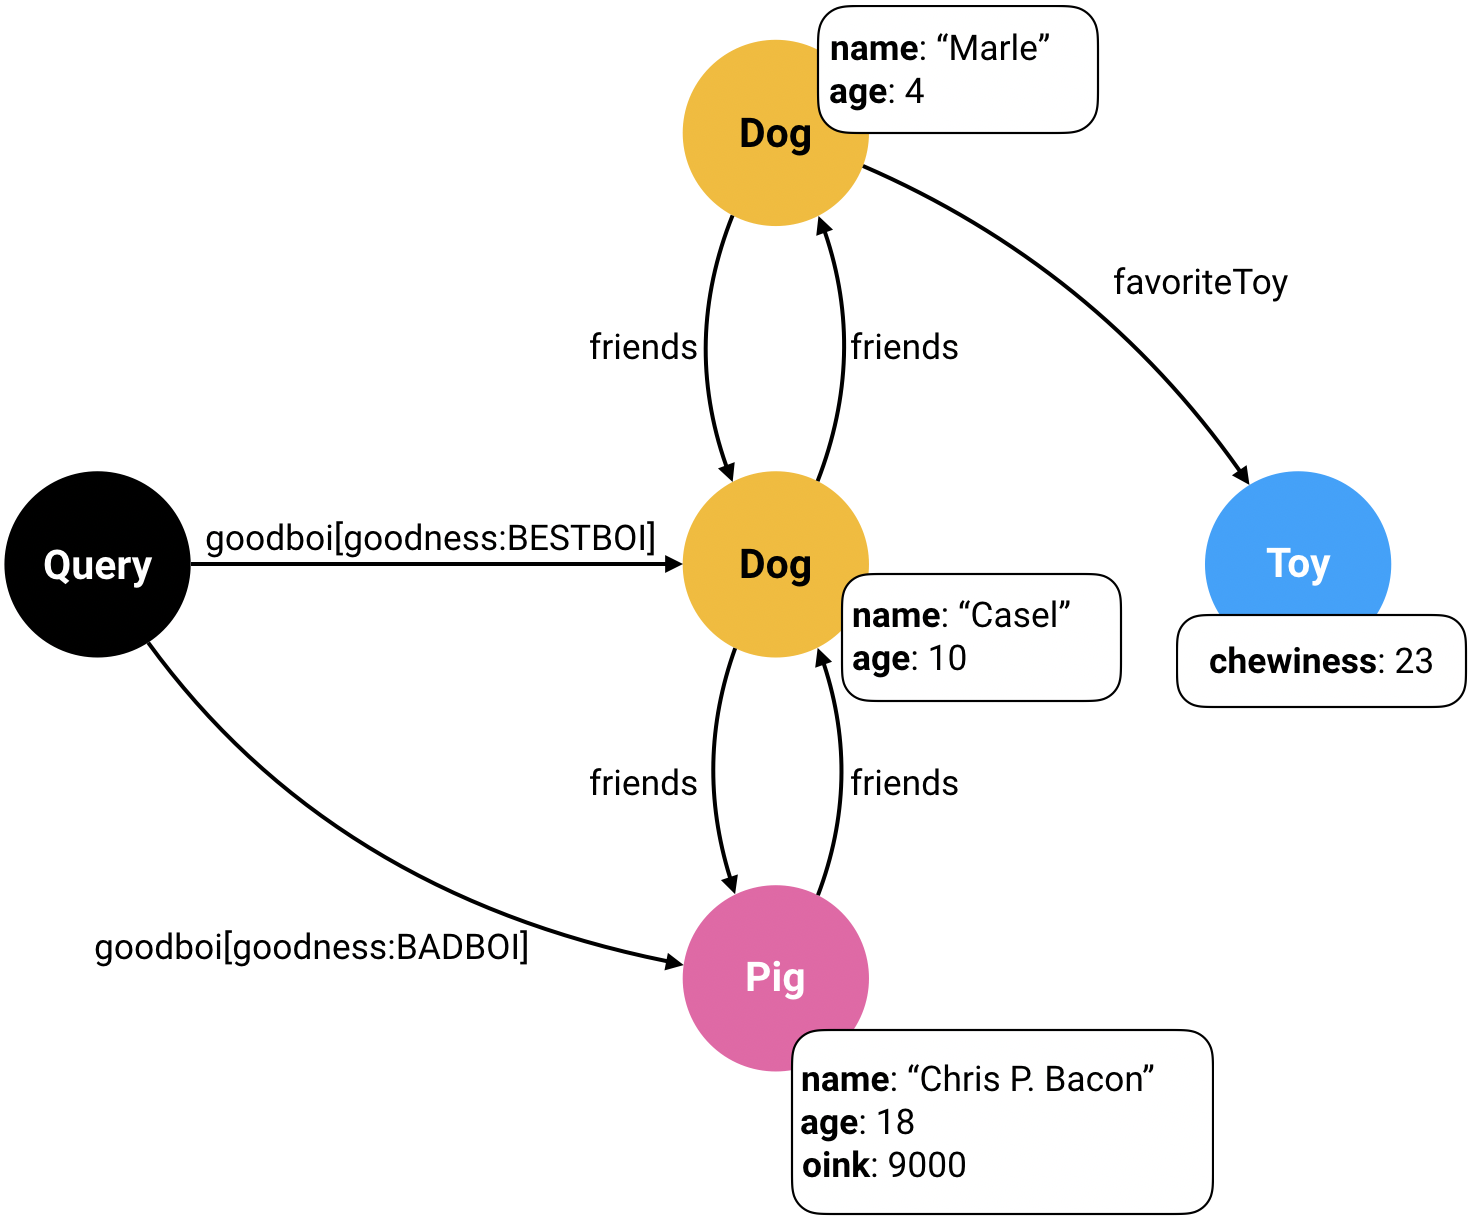
\includegraphics[scale=0.33]{imgs/graph.png}
    \caption{Example of \gql graph.}
    \label{fig:graph_ex}
\end{figure}

%Finally, now that we have defined our type system and data, our developers can proceed to query it.

%\fo{The following three paragraphs were moved from \S \ref{subsec:graph} and should
%be integrated into this section.} An important aspect of \gql is that it is not tied to any particular database technology and implementation. When resolving queries, \gql simply assumes the existence of \textit{resolvers}, which are internal functions defined by the user implementing a \gql service. They are not tied to any particular data model and the only requirement is that they must adhere to the schema. It is up to the user whether the resolvers access a database, return static values or even modify existing data\footnote{The \spec{} states that resolvers ``\textit{must always be side effect‐free and idempotent}'' but the definition of a resolver does not actually impose these restrictions.}. This looseness makes it hard to reason about the semantics.

%With this in mind, we choose to follow \HP's approach and define the underlying data model as a graph over which queries are evaluated. With this model, the unspecified resolvers can be instantiated to concrete definitions, which allow reasoning over them. The semantics are then described as being implemented over a graph setting. Although this provides benefits when reasoning about the semantics, it also comes with some potentially severe limitations over the completeness of the possible results generated.\td{They may not actually be limitations with the model, but there are open questions on how to model some things.} We provide a more thorough explanation of these in \S\ref{sec:discussion}, as well as \HP's approach to the subject.

%Informally, a \gql graph is a directed property graph, with labeled edges and typed nodes. The graph describes entities with their types and properties, as well as the relationship between them. This means that every node has properties (key-value pairs) and a type. Also, every label in an edge describes the relation between two nodes. Finally, every property or label may also contain a list of arguments (key-value pairs).


\paragraph{\gql query and response.}

With the schema and data defined, it is possible to query the service. 
As previously hinted, \gql queries are performed over the types and fields defined in the schema.
They have a tree structure, similar to \json, which follows the fields and relations established between the types
in the type system.

To illustrate this, we define the query in
Figure~\ref{fig:qres_ex}. Intuitively, we request the name of the best
animal in \goodbois, as well as the name and some additional
information of its friends. The query starts by selecting the field
\texttt{goodboi} of the \texttt{Query} type and providing the argument
\texttt{BESTBOI}. The type of this field is the interface
\texttt{Animal}, therefore the query continues selecting the field
\texttt{name}, with scalar type \texttt{String}, and the field
\texttt{friends}, with type \texttt{[Animal]}.  Because the interface
type \texttt{Animal} is implemented by two different object types,
namely \texttt{Dog} and \texttt{Pig}, one can use more specific
selections to further specify the fields that should be requested for
each concrete type. This is achieved by the pair of selections
\ifrag{Dog}{\texttt{favoriteToy \{ chewiness \} }} and \ifrag{Pig}{
  \texttt{loudness:oink} }, which indicate that in the case of a 
dog, the query should request information about field
\texttt{favoriteToy}, while in the case of a pig, the query should
retrieve field \texttt{oink}. In this case, the field selection
\texttt{loudness:oink} indicates that, instead of using the original
field name \texttt{oink}, the resulting value should
be renamed to \texttt{loudness} in the response. %\fo{Maybe introduce here ``inline
%  fragment'', ``selection'', etc.}

This query is then evaluated over the graph, resulting in the response
depicted on the right of Figure~\ref{fig:qres_ex}, which closely
resembles the query.  The intuition behind the evaluation process is
that the query indicates what edges to traverse in the graph and what
properties to access on each node. In this manner, starting from the
node with type \texttt{Query}, the field \texttt{goodboi(goodness:
  BESTBOI)} indicates that the evaluation should continue in an
adjacent node reached after traversing an edge whose label matches the
field. The first step then takes the evaluation process to the central
node, of type \texttt{Dog}.  From there, the query accesses the value
of the node's property matching the field \texttt{name} and then
continues navigating the graph in search of the dog's friends.

%As previously mentioned, the queries we perform over our system must be over the types and fields defined in the schema. Every query must start by requesting information from the \texttt{Query} type. That means that, in our setting, queries must all start with the \texttt{goodness} or \texttt{search} fields.

%In figure \ref{fig:qres_ex}, we can see a query where we asking for all the friends of the \texttt{BESTBOI} in our system. For each friend we ask for their \texttt{name}. The query can be further specified, using fragments, and say that for the \texttt{Dog} friends we want to know their toy's \texttt{chewiness} and for the \texttt{Pig} friends, their \texttt{oink} level. We rename this last selection to \texttt{loudness}. As we can see from this example, queries in \gql have a tree structure similar to \json.

%If we evaluate this query in the graph depicted in \ref{fig:graph_ex}, we would get the response shown in figure \ref{fig:qres_ex}. This response was obtained by navigating the graph and collecting the information contained in each of the relevant nodes. It is easy to see that the response has a structure very similar to the query's.


\begin{figure}
\centering
\begin{subfigure}{.25\textwidth}
\begin{minted}[fontsize=\scriptsize, escapeinside=||,mathescape=true]{js}
query {
  goodboi(goodness:BESTBOI) {
    name
    friends {
      name
      |$\ldots$| on Dog {
        favoriteToy {
          chewiness
        }
      }
      |$\ldots$| on Pig {
        loudness:oink
      }
    }
  }
}
\end{minted}
\label{fig:query_ex}
\end{subfigure}%
\begin{subfigure}{.25\textwidth}
\begin{minted}[fontsize=\scriptsize]{json}
{
  "goodboi": {
    "name":"Casel",
    "friends":[
      {
        "name": "Marle",
        "favoriteToy": {
          "chewiness": 23
        },
      },
      {
        "name": "Chris P. Bacon",
        "loudness": 9000
      }
    ]
  }
}
\end{minted}
\label{fig:response_ex}
\end{subfigure}

\caption{Example of \gql query (left) and its response (right).}
\label{fig:qres_ex}
\end{figure}

\td{We can probably skip this paragraph to save space}
As a final note, one of the appeals of \gql is that if we change our minds and no longer wish to request the friends's names, it would only suffice to remove the field selection 
\texttt{name} from the \texttt{friends} subselections, and the generated response would no longer contain that piece of information. Similarly, reordering the output is simply done
by reordering the selections in the query.
We would not be required to define a new endpoint nor we would get
information we no longer needed, as is usual the case with RESTful
services. 


%If we wanted to ask another the same query but now without the friends' names, we would only have to remove the \texttt{name} field and \textit{voilà}, that's it. We use the same endpoint as before and the \gql service handles the resolution of our fields.

This concludes our brief introduction to \gql and we can now move onto the formalization.
The key points to take from our example are that in order to define a \gql service it is necessary to define the schema, describing the service's type system,
to which the underlying data model and the queries must adhere. \gql queries are selections over fields and types defined in the schema, and their responses closely match 
the queries tree structure.
